\section{含噪观测}
\label{sec:bo-noisy}

到目前为止，读数都是函数值本身。真实的仿真或实验常常带噪声，同一个$\bm{x}$运行两次，结果不一样。设
\begin{equation}
 y_i=f(\bm{x}_i)+\varepsilon_i,
 \label{eq:bo-noisy-obs}
\end{equation}
其中$\varepsilon_i$相互独立，服从均值为$0$、方差为$\tau^2$的高斯分布。此时要分清两个对象：未知但固定的函数值$f(\bm{x})$，和每次测量才产生的随机读数$y$。这就需要回答：噪声使前面哪些做法失效，选点规则应当怎样改？

\subsection{两种预测方差}
\label{sec:bo-noise-variances}

噪声出现后，“这个位置的不确定性”有两种说法。一种是对潜在函数值$F(\bm{x})$的不确定，后验方差为$s_t^2(\bm{x})$。另一种是对下一次读数$y$的不确定，这要多加一份测量噪声。独立噪声方差为$\tau^2$时，
\begin{equation}
 \operatorname{Var}(y\mid\mathcal{D}_t,\bm{x})=s_t^2(\bm{x})+\tau^2.
 \label{eq:bo-pred-var}
\end{equation}
这里用到$y=F(\bm{x})+\varepsilon$，新的$\varepsilon$与$F$及已有数据独立，方差相加。

图~\ref{fig:bo-noise-bands}展示了两者的差别。浅蓝带表示潜在函数值的范围，紫色虚线表示下一次读数可能的范围。读数点不再落在后验均值上，模型会把读数“往回拉”，因为它知道读数里含有噪声；即使在读数附近，后验方差也不为零。

\begin{BookInlineFigure}
 \centering
 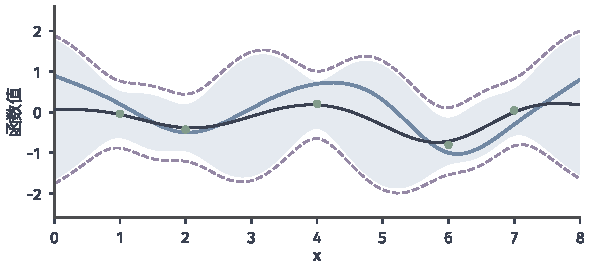
\includegraphics[width=100mm]{figures/05-optimization/05-stochastic-optimization/matplotlib/bo-noise-bands/figure.pdf}
 \caption{两种预测方差。噪声标准差$\tau=0.3$，绿点是五个含噪读数（固定随机种子）。蓝线是目标，深色线是后验均值，浅蓝带是$m_t\pm2s_t$，紫虚线是$m_t\pm2\sqrt{s_t^2+\tau^2}$。}
 \label{fig:bo-noise-bands}
\end{BookInlineFigure}

在同一位置重复读数，能减少的是第一种方差。设先验方差为$1$，$\tau^2=0.09$，在$x$处读$n$次，由定理~\ref{thm:bo-posterior}，
\[
 s^2(x)=\frac{\tau^2}{n+\tau^2}.
\]
$n=1,4,9$时，$s^2$依次约为
\[
 0.083,\qquad 0.022,\qquad 0.010.
\]
而下一次读数的方差始终比$s^2$多$0.09$，这一份噪声不会因观测而消失。观测多了，我们越来越清楚$f(x)$是多少，但下一次测量出来的数照样抖动。

\paragraph{方差能否只减不增}
超参数固定时，由更新式~\eqref{eq:bo-update-cov}，
\[
 s_{t+1}^2(\bm{x})=s_t^2(\bm{x})-\frac{c_t(\bm{x},\bm{x}^+)^2}{s_t^2(\bm{x}^+)+\tau^2}\leq s_t^2(\bm{x}),
\]
新增观测不会使潜在值的后验方差增大。这个结论只在模型固定时成立。

重新拟合超参数就可能使方差增大。设$k=\sigma^2k_0$，其中$k_0$是贯穿例的核，幅度$\sigma^2$用边缘似然估计，无噪声。只有$x=1$的读数$1$时，估计值$\widehat{\sigma}^2=1$，于是
\[
 s^2(2)=\widehat{\sigma}^2\cdot\tfrac34=0.75.
\]
再评价相距很远的$x=6$，读到$3$，两点几乎不相关，幅度估计变为
\[
 \widehat{\sigma}^2\approx\frac{1^2+3^2}{2}=5,
\]
于是$s^2(2)\approx3.75$，反而变大了。新读数告诉模型“函数的波动比原来以为的大”，模型便下调了之前的把握。这两种情形都和“消除下一次测量的噪声”无关。

\subsection{含噪选点}
\label{sec:bo-noisy-selection}

\paragraph{最低读数可能只是运气好}
式~\eqref{eq:bo-incumbent}的$b_t$在含噪时不能直接用读数的最小值代替。读数的最小值常常是噪声偏向负方向的那一次。图~\ref{fig:bo-noise-incumbent}上半部分中，六个读数里最低的是$x=2$处的$-0.95$（红圈），但$f(2)=-0.5$，真实更好的$x=6$只读到$-0.55$，因为那次噪声是正的。

用含噪的最低读数做阈值，会把门槛设得过低，好像已经找到一个其实并不存在的好结果。一种改法是把阈值换成已评价点上的最小后验均值，这样噪声被模型部分平滑了；这是一种具体的近似规则，并不等于对真实阈值作了正确处理。

\paragraph{含噪期望改进}
更一致的做法是承认阈值也不确定。真实的“已评价最好值”是$\min_iF(\bm{x}_i)$，它是随机的。把它和候选点放在同一个后验下，定义\term{含噪期望改进}（noisy expected improvement，NEI）：
\begin{equation}
 \mathrm{NEI}_t(\bm{x})=\mathbb{E}\Bigl[\bigl(\min_{i\leq t}F(\bm{x}_i)-F(\bm{x})\bigr)_+\,\Bigm|\,\mathcal{D}_t\Bigr].
 \label{eq:bo-nei}
\end{equation}
这里的期望对$F(\bm{x}_1),\ldots,F(\bm{x}_t),F(\bm{x})$的\emph{联合}后验取，协方差不能丢：若候选点与某已评价点强相关，两者的差就不会太大。一般情形下没有闭式，常用的做法是抽取这$t+1$个值的联合后验样本，取平均。

\paragraph{例：只有一个评价点}
只有一个评价点时，NEI可以手算。设$\tau^2=0.09$，在$x=2$读到$y=-0.5$，候选为$x=4$。相关系数$\rho=1/16$，由定理~\ref{thm:bo-posterior}，
\[
 \begin{aligned}
 F(2)\mid\mathcal{D}:&\ \text{均值}\ -0.459,\quad\text{方差}\ 0.083,\\
 F(4)\mid\mathcal{D}:&\ \text{均值}\ -0.029,\quad\text{方差}\ 0.996,
 \end{aligned}
\]
两者的后验协方差约为$0.005$。

把$D=F(2)-F(4)$看成一个高斯量，其均值与方差为
\[
 \mathbb{E}D\approx-0.430,\qquad \operatorname{Var}D\approx0.083+0.996-2\times0.005\approx1.069.
\]
由于$\mathrm{NEI}=\mathbb{E}D_+$，用式~\eqref{eq:bo-ei}的同一积分，标准化后$u\approx-0.416$，
\[
 \mathrm{NEI}\approx-0.430\,\Phi(u)+1.034\,\phi(u)\approx0.233.
\]

同一位置上，以读数$-0.5$为阈值的EI约为$0.206$，以后验均值$-0.459$为阈值的EI约为$0.220$。NEI最大，因为它考虑了阈值$F(2)$自身的不确定性：阈值可能比后验均值高，候选点就更容易改进。

图~\ref{fig:bo-noise-incumbent}下半部分比较了三种做法。阈值用最低读数时，门槛被噪声压低，除$x=2$附近外，分数都比另外两条线小（黄线）；阈值用最小后验均值时，$x=2$处仍有一个较高的峰，因为最小后验均值落在$x=2$（紫虚线）；NEI在已评价的$x=2$附近凹下去，并把价值分到其他地方（绿线）。

\begin{BookInlineFigure}
 \centering
 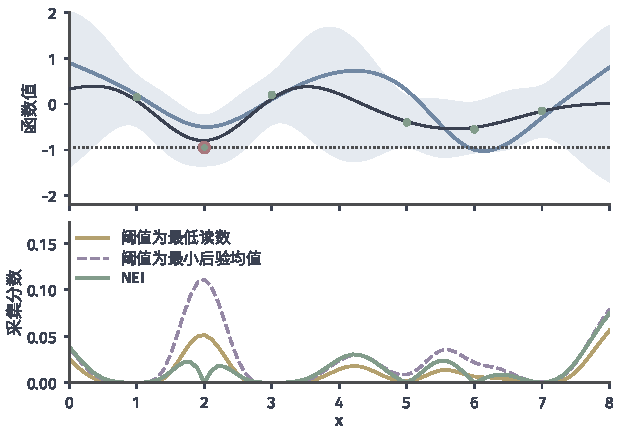
\includegraphics[width=105mm]{figures/05-optimization/05-stochastic-optimization/matplotlib/bo-noise-incumbent/figure.pdf}
 \caption{最低读数与含噪选点。上：$\tau=0.3$，六个读数，噪声依次取为$-0.05,-0.45,0.1,-0.7,0.45,0.15$（手工给定，用以突出$x=2$的偶然低值），红圈是最低读数，点线是其数值；蓝线是目标，深色线是后验均值。下：三种采集分数，NEI由$40000$个联合后验样本估计。}
 \label{fig:bo-noise-incumbent}
\end{BookInlineFigure}

NEI和知识梯度衡量的东西不同。NEI问的是“潜在函数值能否低于已评价点”，KG问的是“这次观测后，最终推荐的价值能改善多少”。无噪声时前者是EI的直接推广，后者需要再做一次前瞻。两者都在含噪时有定义，下一节就会看到它们对“重复测量”的回答相反。

\subsection{重复评价}
\label{sec:bo-replicates}

含噪时一个自然的动作是把同一个位置再测一次。这样做有用吗？按潜在改进的定义，答案是否定的。若$\bm{x}$恰好是某个已评价点$\bm{x}_j$，则$\min_iF(\bm{x}_i)\leq F(\bm{x}_j)$，改进量恒为$0$，所以
\begin{equation}
 \mathrm{NEI}_t(\bm{x}_j)=0.
 \label{eq:bo-nei-zero}
\end{equation}
图~\ref{fig:bo-noise-incumbent}的绿线在$x=2$处贴到零，正是这个原因。NEI从定义上就看不到复测的价值，因为复测不产生新位置，只是更清楚地认识旧位置。

复测的价值要由信息更新的准则来衡量。式~\eqref{eq:bo-kg}的KG没有这种限制。设两个候选A、B，$F(\text{A})$的后验均值$0$，方差$s^2=0.04$，$F(\text{B})$的后验均值$0.1$，两者后验独立，测量噪声$\tau^2=0.09$。当前推荐A。再测一次A后，由式~\eqref{eq:bo-kg-update}，
\[
 \widetilde{\sigma}=\frac{0.04}{\sqrt{0.04+0.09}}\approx0.111.
\]

新的推荐价值是$\min\{0.111Z,\ 0.1\}$，标准化的间距$u=0.1/0.111\approx0.901$。于是
\[
 \begin{aligned}
 \mathrm{KG}&=0-\mathbb{E}\min\{0.111Z,\,0.1\}\\
 &=0.111\bigl(\phi(u)-u(1-\Phi(u))\bigr)\approx0.011.
 \end{aligned}
\]
这个值大于$0$：再测一次A可能发现它其实比B差，从而改变推荐。

\paragraph{该重复多少次}
重复次数取决于要区分的差距和噪声。设两个候选的真实差距为$\Delta$，噪声标准差为$\tau$，各读$n$次后比较平均读数，选对的概率为
\begin{equation}
 \mathbb{P}(\text{选对})=\Phi\left(\frac{\Delta\sqrt{n}}{\tau\sqrt{2}}\right).
 \label{eq:bo-correct-selection}
\end{equation}
这里用到两个平均读数之差服从$N(\Delta,2\tau^2/n)$。取$\Delta=0.2$，$\tau=0.3$，$n=1,4,9$时的概率依次为
\[
 0.681,\qquad 0.827,\qquad 0.921.
\]
可见差距接近噪声水平时，一次测量基本在碰运气。代价接近的候选之间要靠复测来决定，能否负担这个复测要由预算决定。

最后要留意单次异常读数。一个比预期低$3$倍标准差的读数，可能是噪声，也可能是模型错了，比如该位置附近有一个模型没想到的窄谷。留一残差~\eqref{eq:bo-loo}只能发现它异常，不能告诉我们原因。在同一位置复测可以帮助区分：回到预期附近，说明是噪声；复测仍然很低，说明应当修改模型的设定。
